\subsection{Minimum time to climb}

\noindent The current task is to find using trial and error methods, the minimum time 
to reach certain goals. To investigate the situation more thoroughly 
in each try we plot the total energy lines as well as plots for the fuel consumption
the speed of the airplane the height and the $\gamma$ angle.

\subsection{Computing $\gamma(t)$  - minimum time for Mach = 1.5 \& h = 1.1km}
\label{sec:m15h11}

The feasible solution to the above challenge is shown in \ref{fig:m15h11}. \ref{fig:m15h11_2}
is also presented to show the changes of the different properties during the time of flight

\begin{figure}[H]
    \centering
    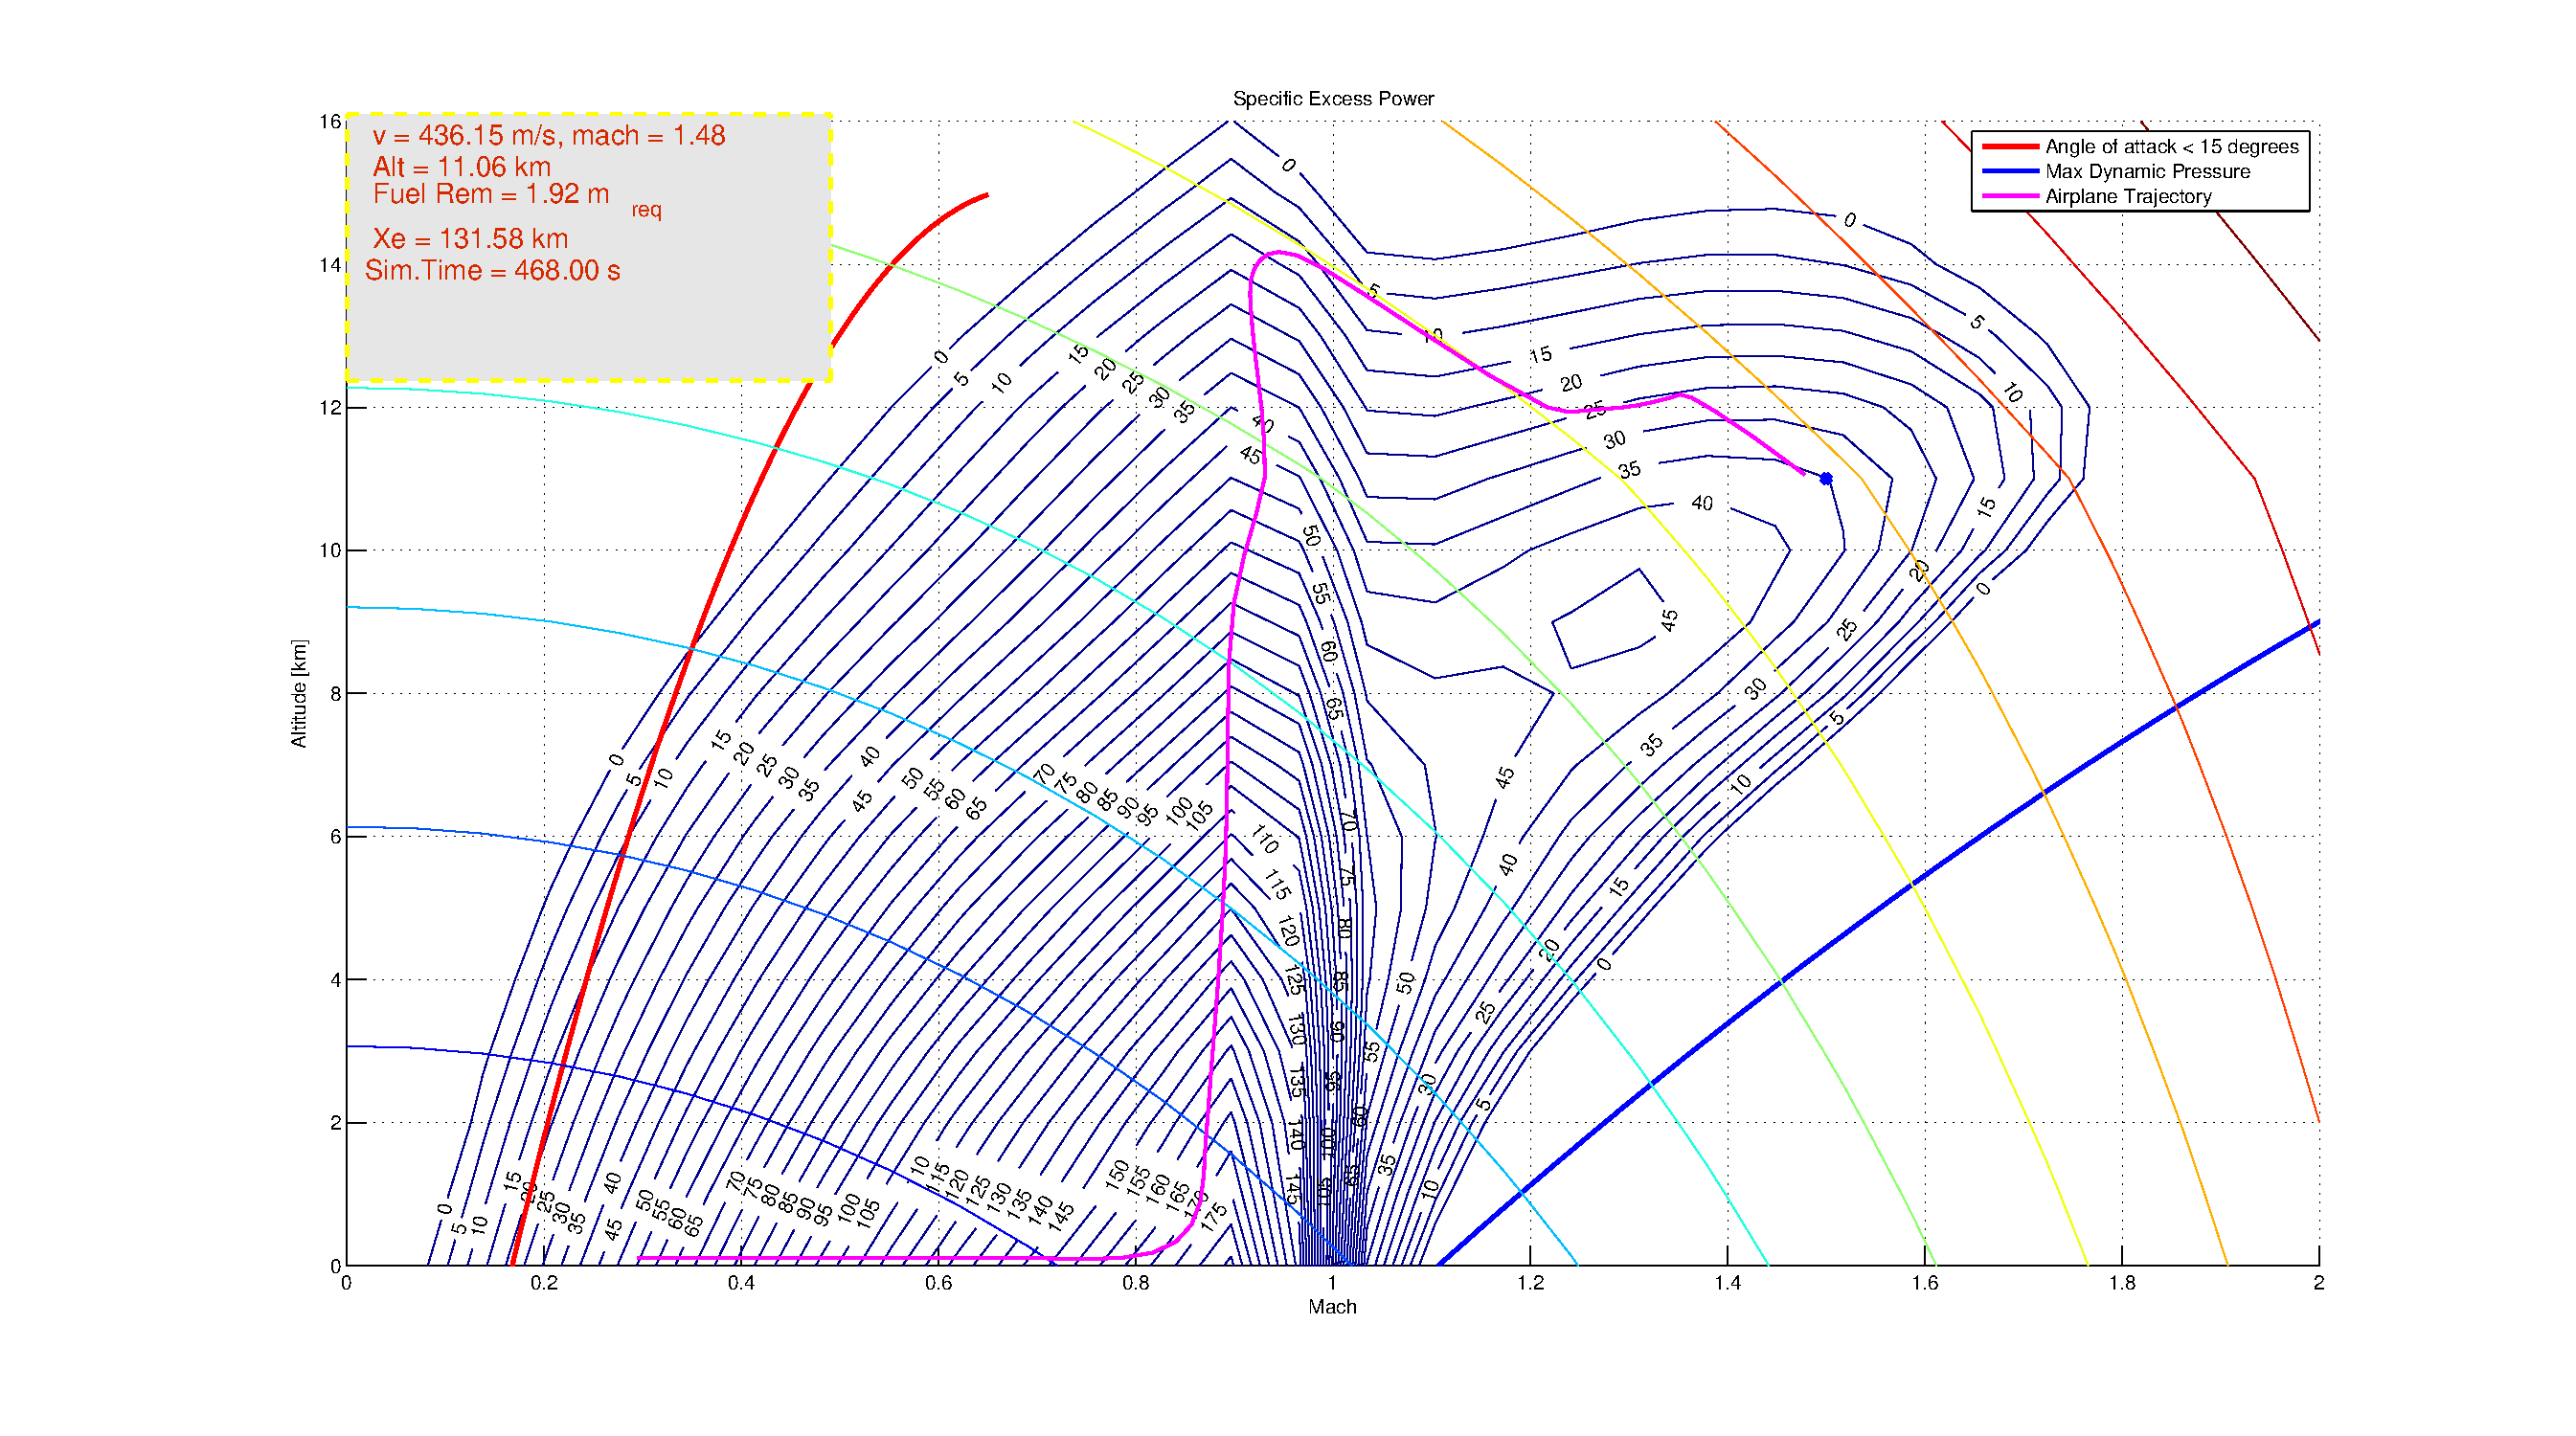
\includegraphics[width=1.0\textwidth]{mach15alt11}
    \caption{Trajector of the airplane to reach M = 1.5 \& h = 11km}
    \label{fig:m15h11}
\end{figure}

\begin{figure}[H]
    \centering
    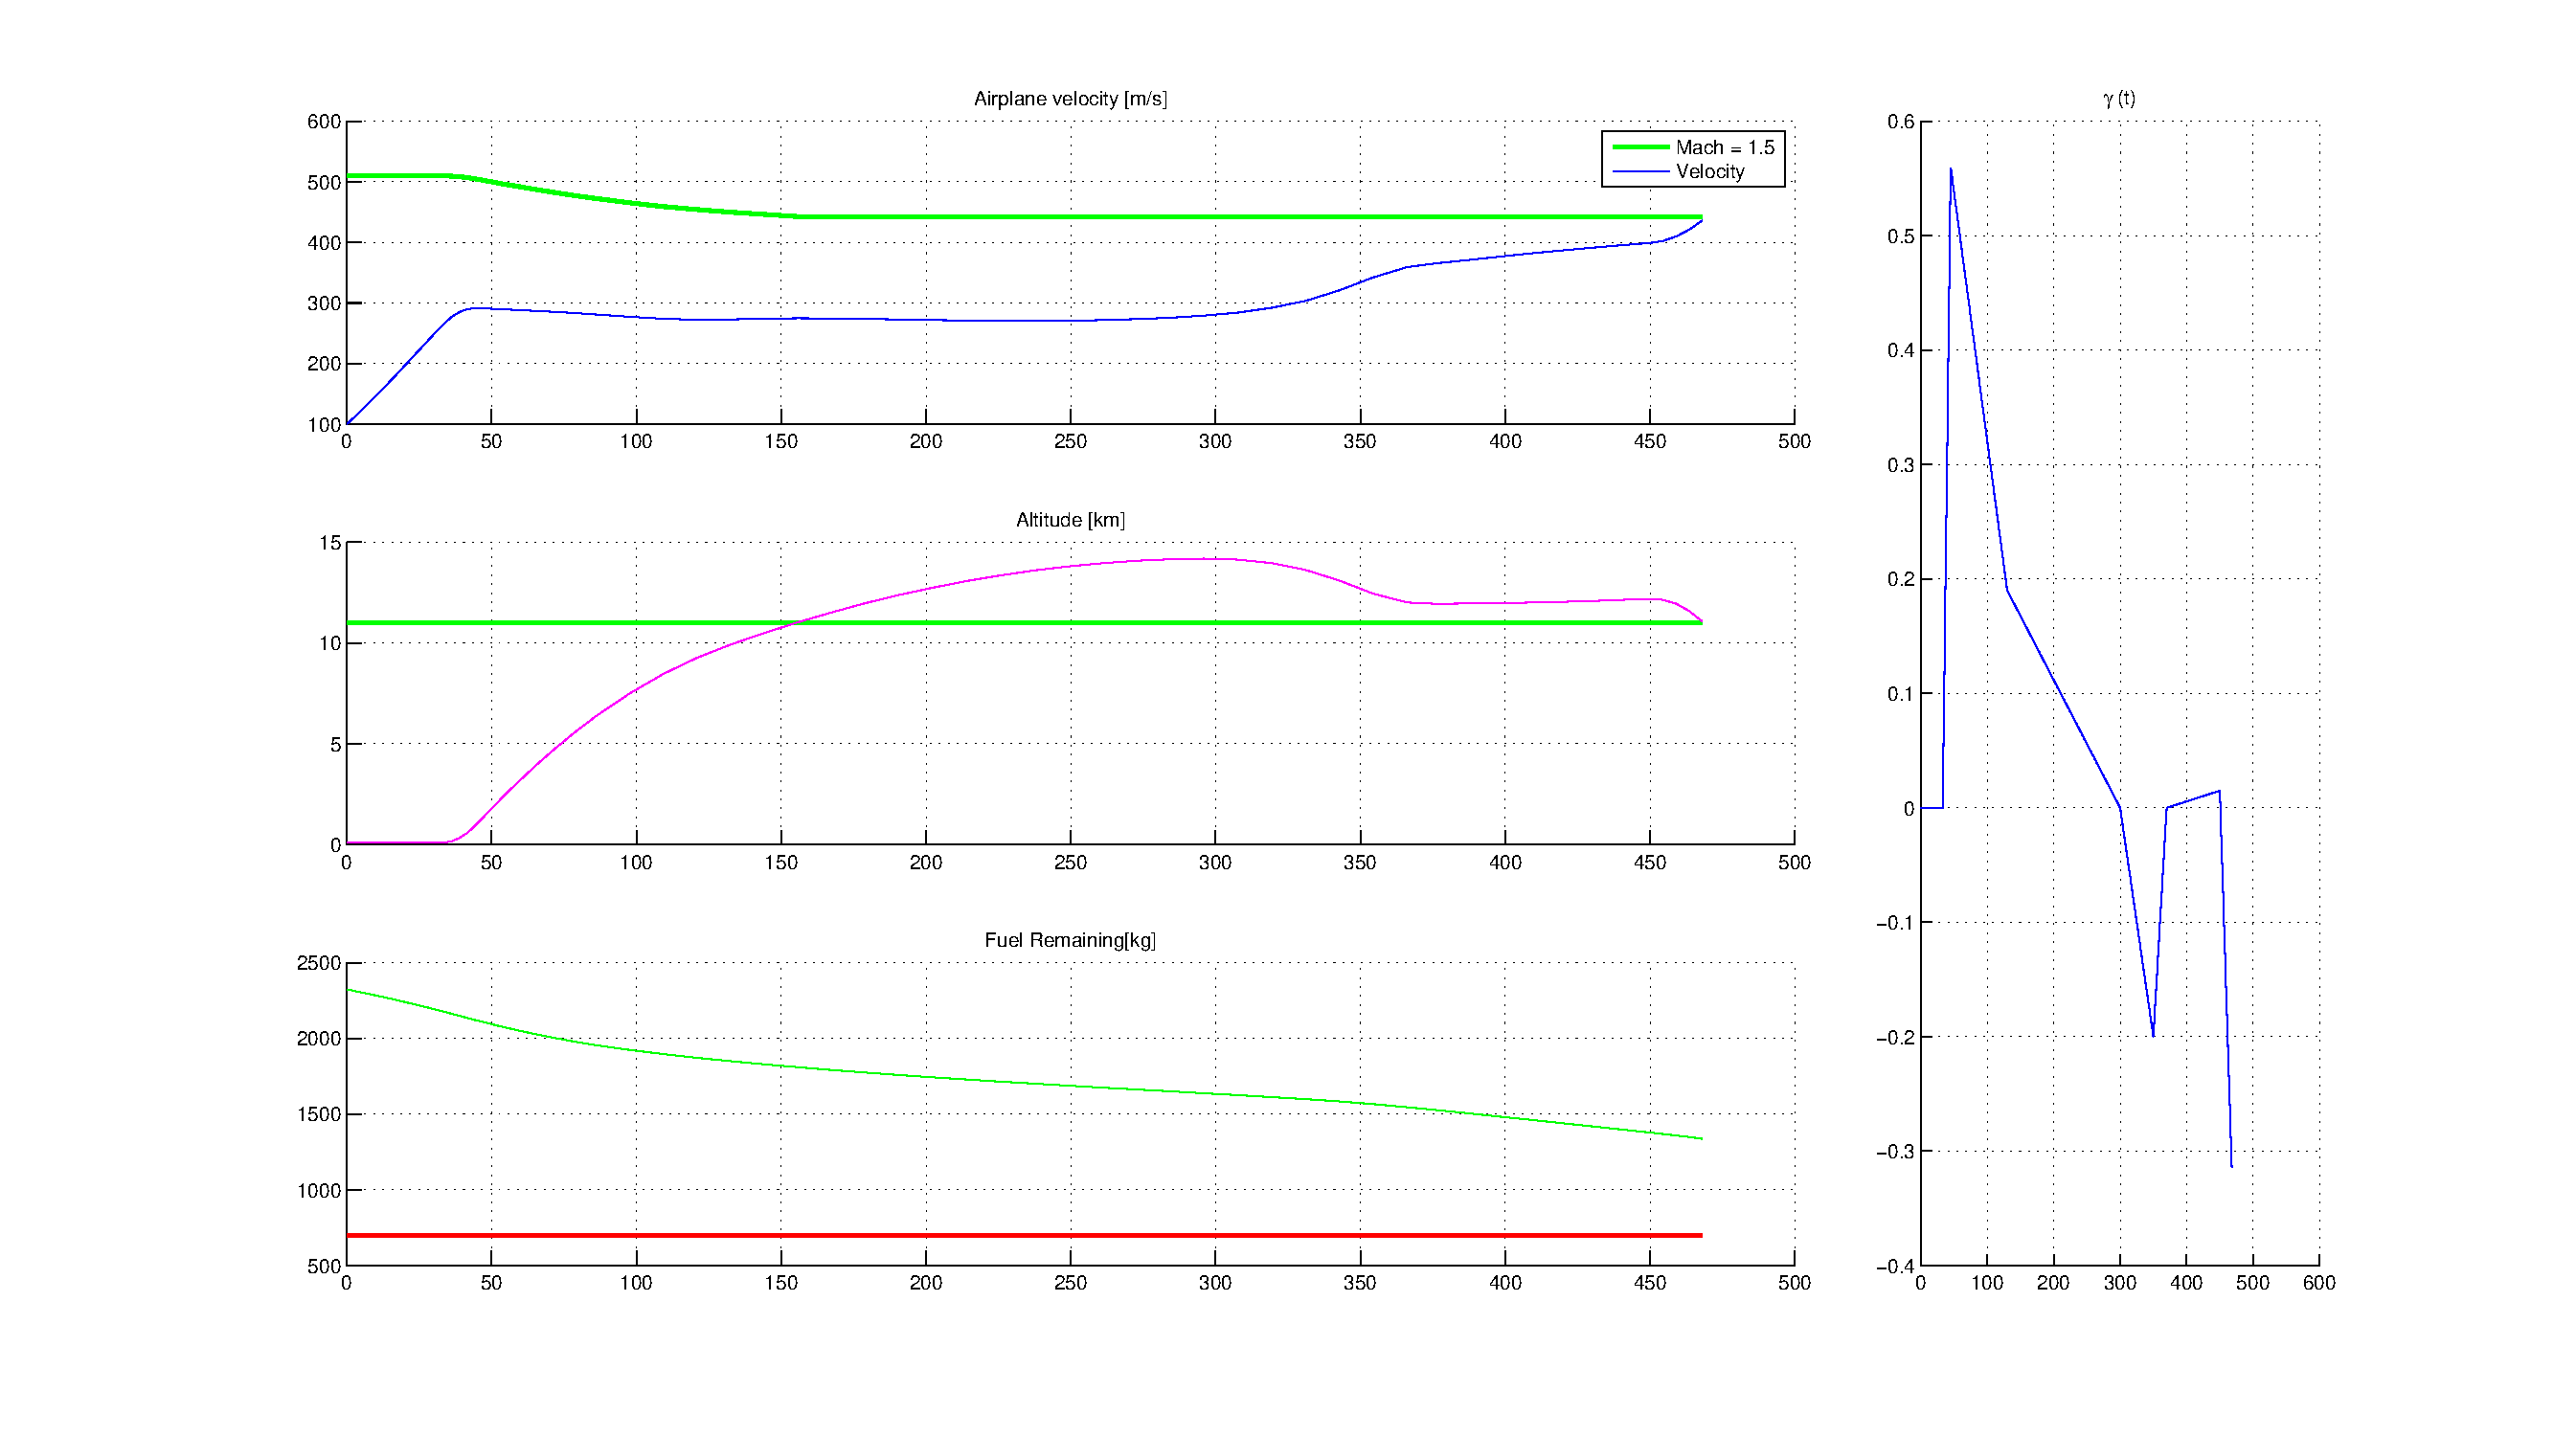
\includegraphics[width=1.0\textwidth]{mach15alt11_2}
    \caption{Velocity, height fuel consumption and $\gamma$ angle during the flight}
    \label{fig:m15h11_2}
\end{figure}

The strategy of the climb is first to climb to higher altitude than needed and then
dive into the supersonic area "with the same slope as an energy line" to
lose the least amount of energy during the manuever.
As we see  the aircraft reaches the goal after 468 seconds which is acceptable both in terms of 
fuel consumption and afterburner time of use.


\subsection{Trajectory for maximum Mach number in minimum time}
To reach the maximum Mach number given by the SEP graph we use the same
strategy as in \ref{sec:m15h11}. The diagram \ref{fig:max_mach} corresponding to the flight are also given below:

\begin{figure}[H]
    \centering
    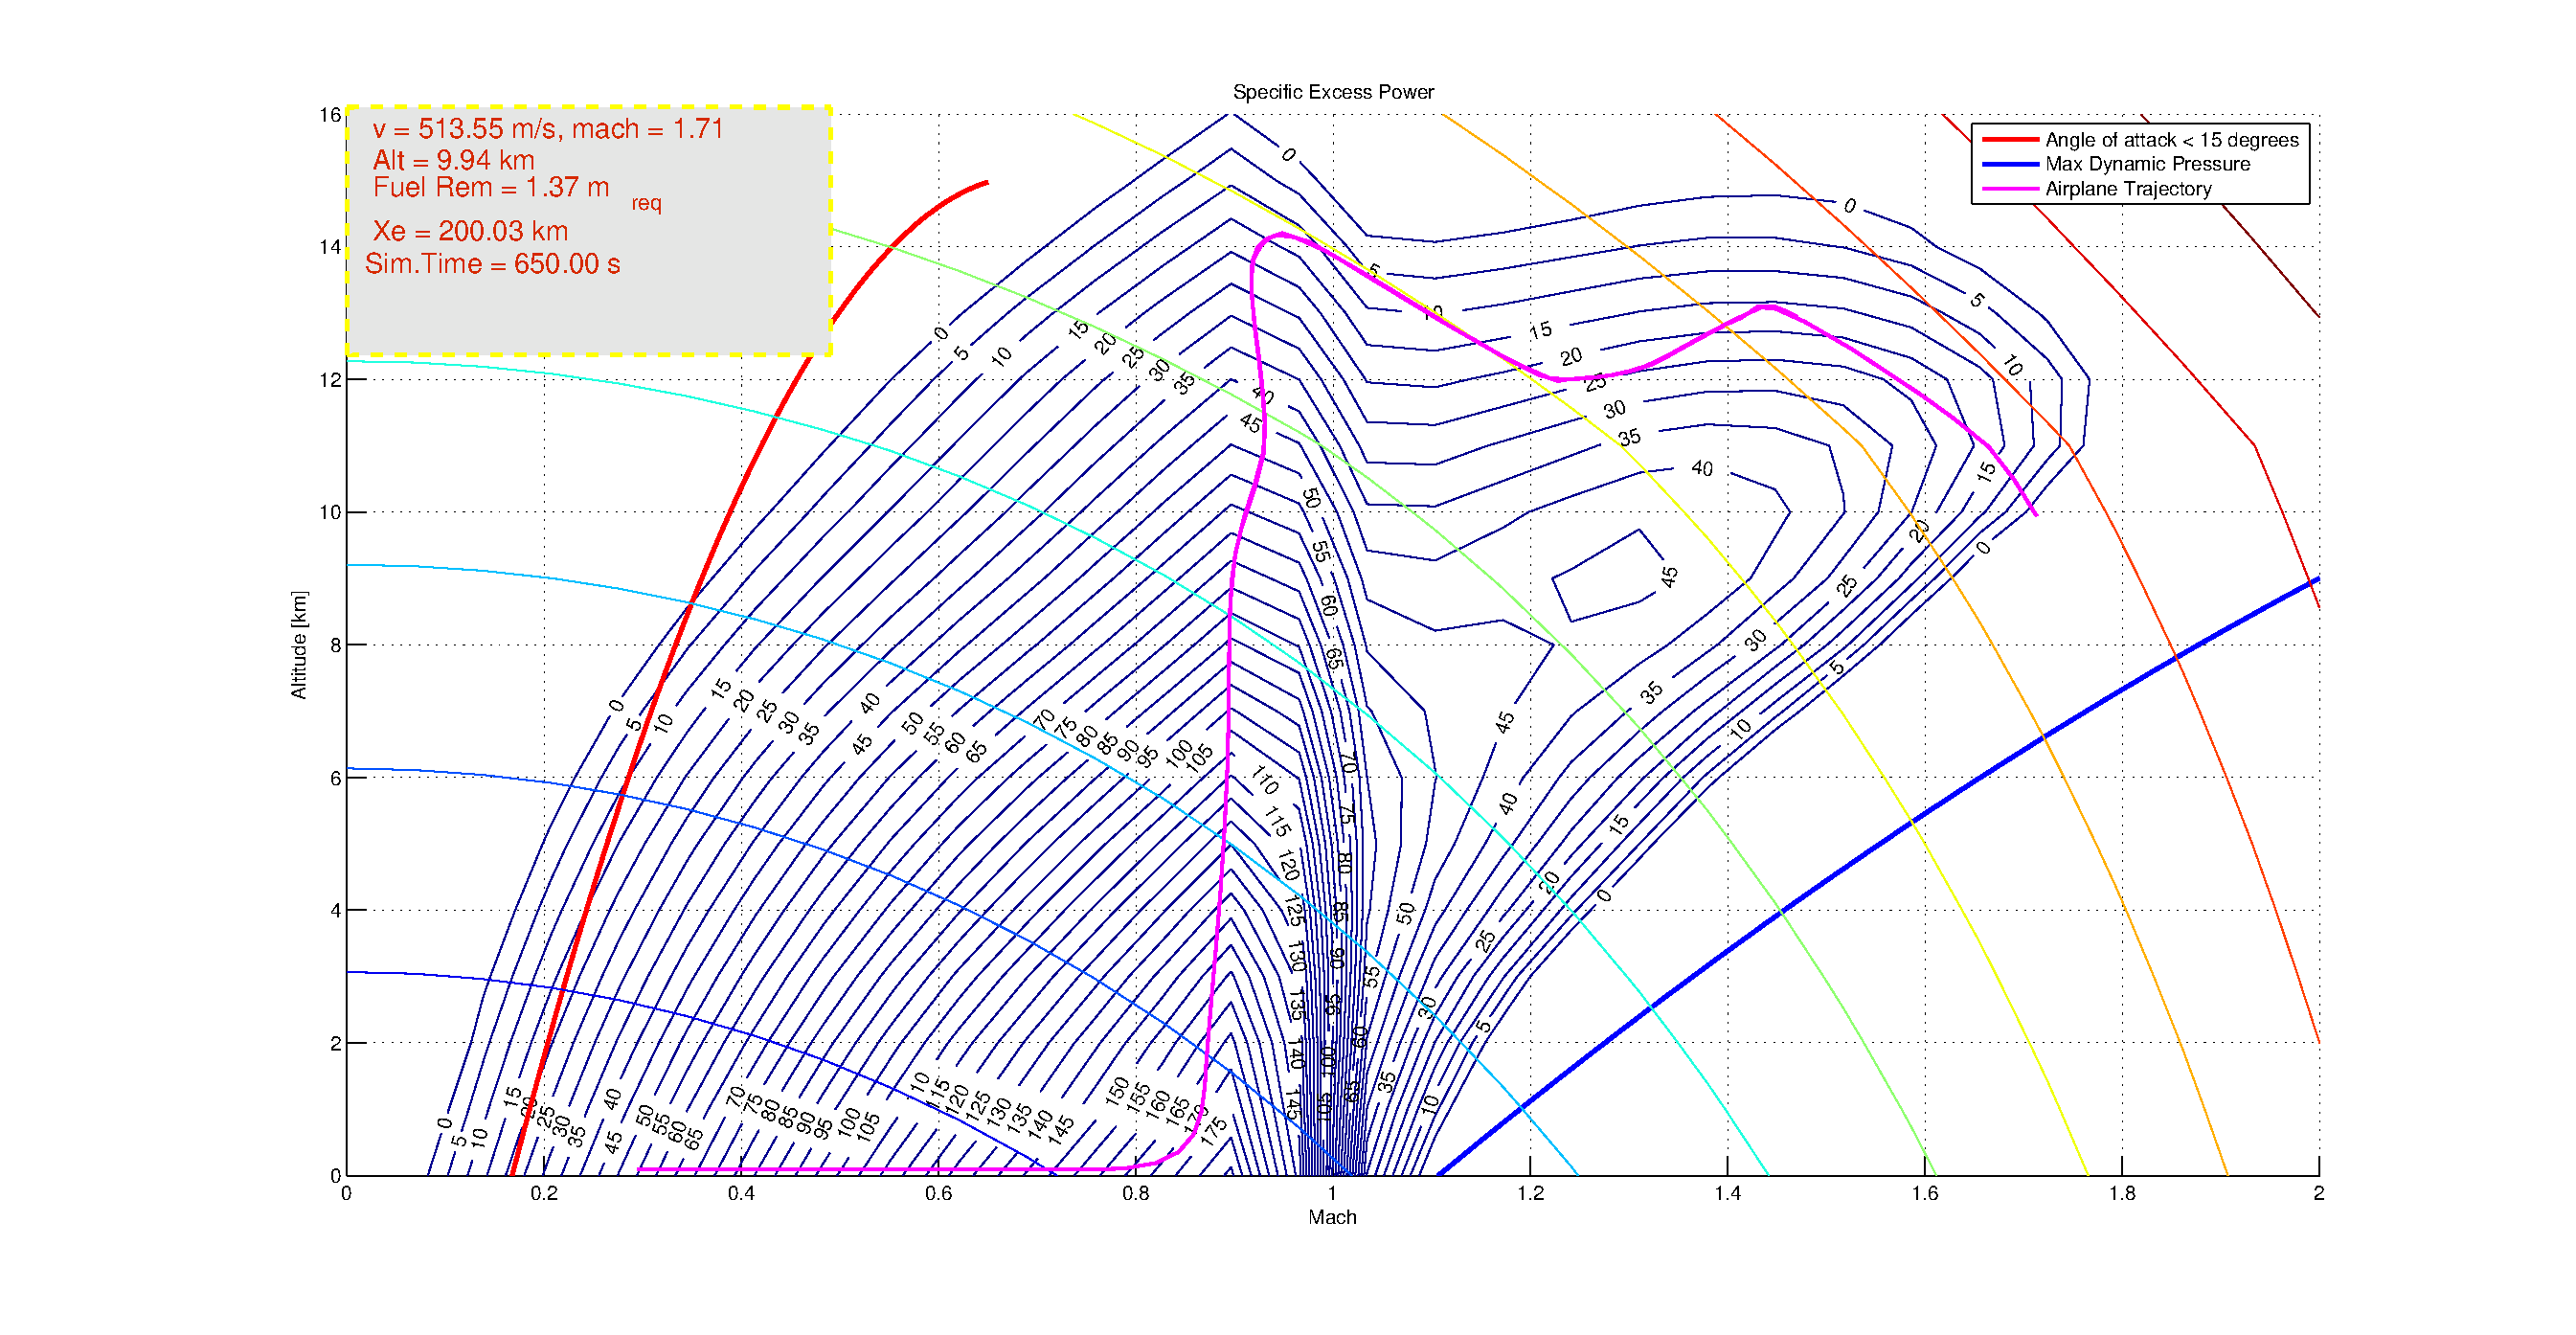
\includegraphics[width=1.0\textwidth]{max_mach}
    \caption{Trajector of the airplane to reach M = 1.76}
    \label{fig:max_mach}
\end{figure}

\subsection{Trajectory for maximum altitude in minimum time}
The diagram for reaching the maximum altitude is given in \ref{fig:max_alt_first_try}.
It is visible that the trajectory is not the best possible as the aircraft reaches a maximum of 15.4 km
instead of the actual goal which is 16km.

\begin{figure}[H]
    \hspace*{-1cm}
    \centering
    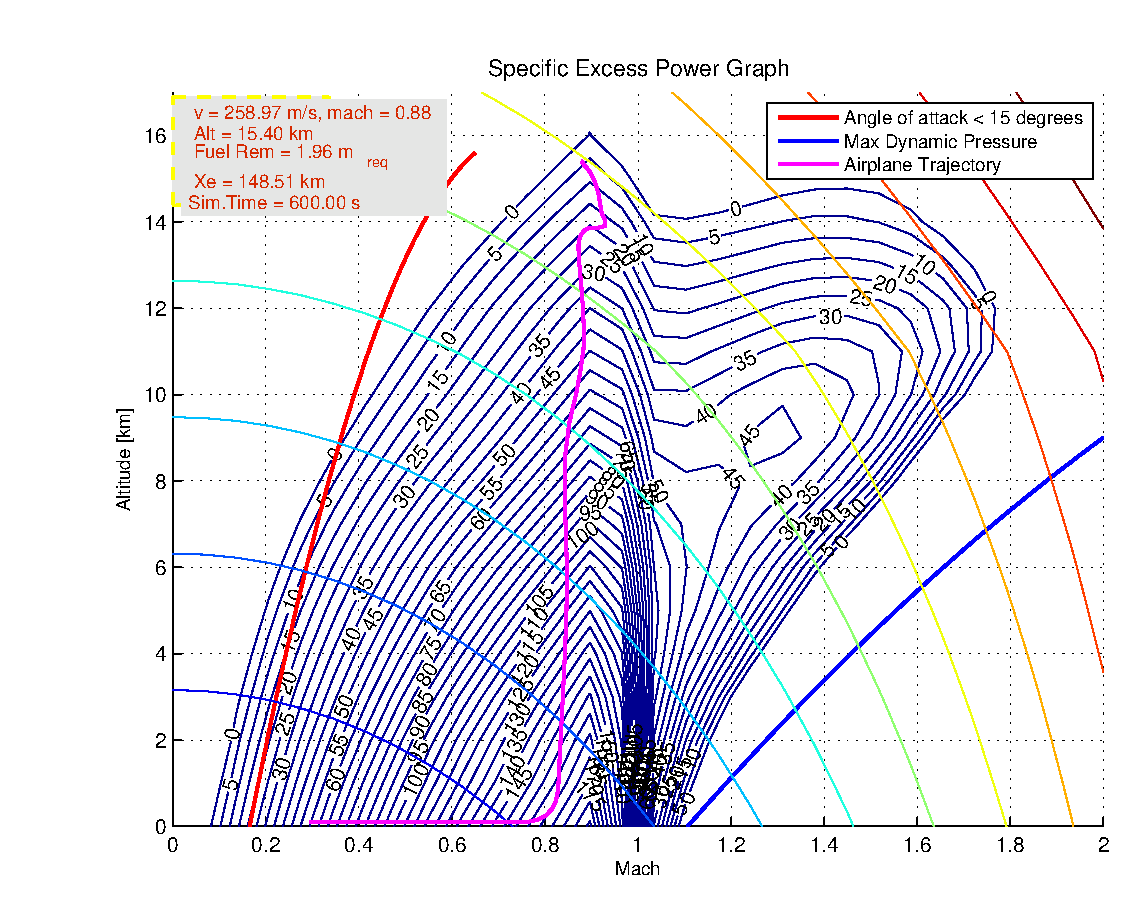
\includegraphics[width=0.8\textwidth]{max_alt_first_try}
    \caption{Trajector of the airplane to reach h = 16km}
    \label{fig:max_alt_first_try}
\end{figure}
